\begin{figure}[h]
    \centering
    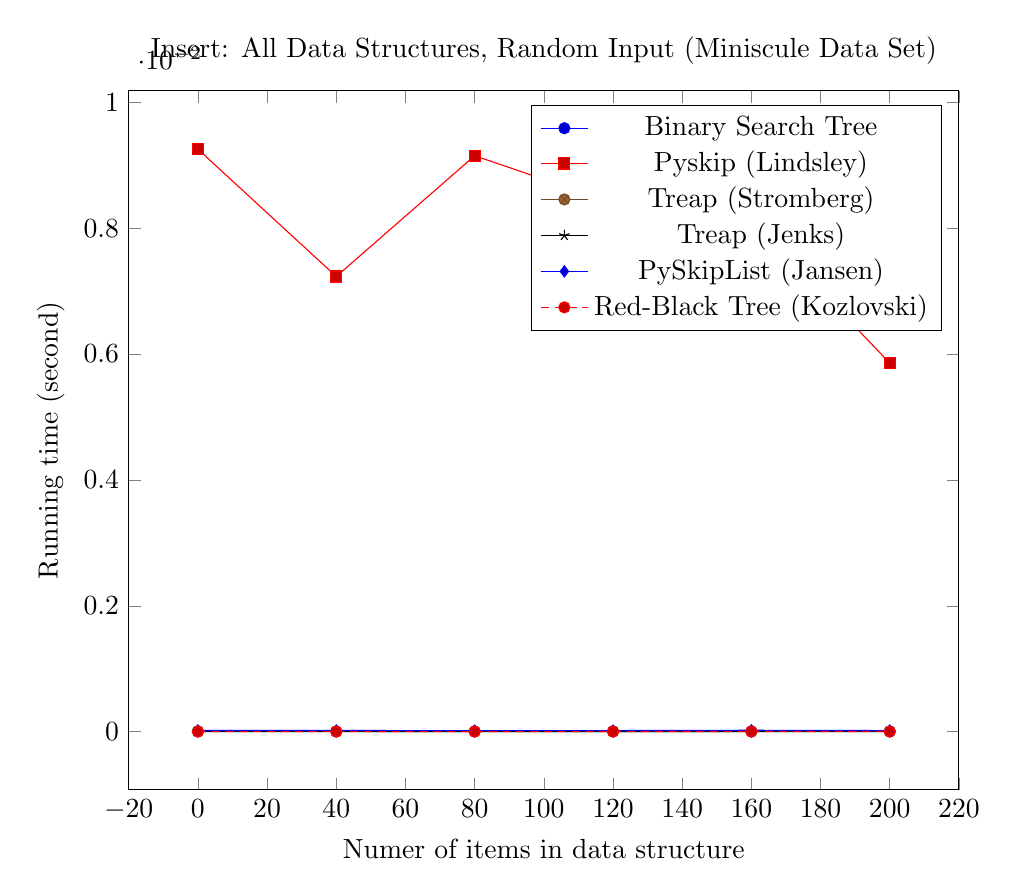
\begin{tikzpicture}
        \begin{axis}[
            xlabel={Numer of items in data structure},
            ylabel={Running time (second)},
            title={Insert: All Data Structures, Random Input (Miniscule Data Set)},
            width=\textwidth
        ]
		\addplot coordinates {
			(0, 5.57174372985969e-06)
			(40, 5.752448931950483e-06)
			(80, 5.270568393189734e-06)
			(120, 6.0536242687092566e-06)
			(160, 5.842801532995878e-06)
			(200, 6.0536242687092566e-06)
		};
		\addplot coordinates {
			(0, 0.009253461634026827)
			(40, 0.007231521010744401)
			(80, 0.009149164614909644)
			(120, 0.008401225783620524)
			(160, 0.008159502458343581)
			(200, 0.005856444775737301)
		};
		\addplot coordinates {
			(0, 7.890793822795672e-06)
			(40, 5.300685926812321e-06)
			(80, 4.306807315579419e-06)
			(120, 4.427277450247402e-06)
			(160, 5.180215792144338e-06)
			(200, 5.300685926812321e-06)
		};
		\addplot coordinates {
			(0, 2.680460497117565e-06)
			(40, 2.4094026938925594e-06)
			(80, 4.005631978820645e-06)
			(120, 2.3190500929359813e-06)
			(160, 2.0781098236000163e-06)
			(200, 2.590107896160987e-06)
		};
		\addplot coordinates {
			(0, 2.08413333030677e-05)
			(40, 2.0148630028593573e-05)
			(80, 1.773922733452338e-05)
			(120, 1.8853576080779533e-05)
			(160, 2.370249900245369e-05)
			(200, 1.8582518277554526e-05)
		};
		\addplot coordinates {
			(0, 2.7105780306513337e-06)
			(40, 2.9515183001649346e-06)
			(80, 3.102105968544322e-06)
			(120, 3.4936339062596743e-06)
			(160, 3.4936339062596743e-06)
			(200, 3.433398839014501e-06)
		};
        \legend{Binary Search Tree, Pyskip (Lindsley), Treap (Stromberg), Treap (Jenks), PySkipList (Jansen), Red-Black Tree (Kozlovski)}
        \end{axis}
    \end{tikzpicture}
    \caption{Average of 10 operations, benchmarked every 40, starting at 0.}
\end{figure}